\section{Overview}

The world is progressing fast enough on technology in the last years and computer science is not an area that falls behind. Computer science can be divided into many areas of study, but we can divide them into three big fields. Software development, information technology and security. We will be focusing on information technology such as artificial intelligence, machine learning and deep learning. In computer science, Artificial Intelligence (AI) is the intelligence carried out by machines. Its goal is to build smart machines capable of performing tasks that normally are made by humans. AI is just software; it is an application written to do a task. For example, on Facebook with suggestions of names of people to tag on pictures, for fraud detection on credit cards or for self- driving cars that can manage their shelves to drive through the city.

As use of AI and deep learning become popular many fields start using these methods to improve many important fields. A vehicular automation system is one of them which is becoming popular recently to create an auto driving car, to detect cars on the road and also making improvements in urban designing for roads. 


\section{Motivation}
Intelligent vehicle detection and vehicle counting are becoming increasingly important in the field of vehicular automation. However, due to the different types of vehicles, their detection remains a challenge that directly affects the accuracy of vehicle classification and detection. Much research has been conducted in this field of vehicular automation but it is mostly done in Europe, America and  other rich countries. Unfortunately this kind of research is new from the perspective of Bangladesh and every country contains different sets of vehicles which is why it is hard to conduct research in these fields. 
\begin{figure}[ht]
    \centering
    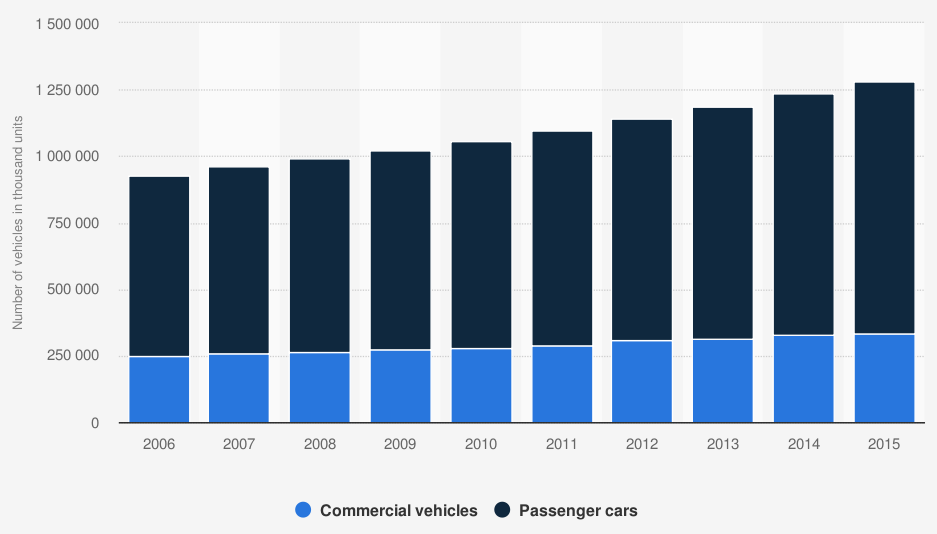
\includegraphics[max width=\textwidth]{images/ours/statistic_id281134_number-of-vehicles-in-use-worldwide-2006-2015.png}
   \caption[World Vehicles in operations]{ World Vehicles in operations \cite{vehicleinoperation}}
    \label{fig:world_vehicle_stat}
\end{figure}
Each year the number of vehicles is increasing and keeping track of them is getting harder. From automatic cars to designing the modern road, we need information related to vehicles. For this, detecting vehicles is important. We know that it is hard but using deep learning and other modern methods for detecting objects we tried to challenge this task. 

\newpage

\section{Research Questions}
This thesis research questions are focused on vehicle detection and it's future. The main research questions are described below:

\begin{itemize}
    \item \textbf{Research Question 1:}  How can we propose a better deep learning model to detect different types of vehicle?

    \item \textbf{Research Question 2: } How can we more accurately classify different types of vehicle and increase classification accuracy?

    \item \textbf{Research Question 3:} How can we improve existing vehicle counting methods?

\end{itemize}

\section{Objectives}
The goal of this study is to build a methodology to detect vehicles from the road of Bangladesh with improved methods which will also solve the vehicles counting problem. Our work is to find a better solution than the existing method which will give better results on our custom dataset.
\begin{itemize}
    \item To propose a better deep learning based model to detect different types of vehicles.

    \item To classify different types of vehicles precisely and increase classification accuracy significantly. 

    \item To count different types of vehicle authentically with precise aim.

\end{itemize}
\newpage
\section{Organization}

The remainder of this research is organized as follows:
   
   \begin{itemize}
       
       \item\textbf{Chapter 2 Related Works}  Highlights the previous research works on vehicles detection system.
       
        \item\textbf{Chapter 3 Object Detection With YOLOv5} Describing how YOLOv5 model works and how it detect objects using deep learning. 
       
        \item\textbf{Chapter 4 Methodology} Illustrates our proposed method with proper example and diagrams. 
       
       \item\textbf{Chapter 5 Result Analysis and Discussion} Results of our proposed method and analysis regarding it.
       
       \item\textbf{Chapter 6 Conclusion and Future Work} Concludes the whole research work and focuses on future research directions.
       
       
       
   \end{itemize}




























 